\chapter{Alcances de la Memoria}
\label{alcances}

\section{Problema a resolver}

Actualmente Chile no cuenta con plantas de energía solar fotovoltaica conectadas a sus redes centrales de distribución (\gloss{SIC}, \gloss{SING}, \gloss{SM}, \gloss{SA}), debido a problemas legales y de normativas técnicas. La mayoría de las plantas solares que generan energía en chile son plantas aisladas o conectadas a sistemas de distribución privados, como por ejemplo Calama Solar 3\cite{plantaSolar:1} y Subsole\cite{subsole:2}.

La Red Solar para Latinoamérica y el Caribe (RedSolLac), tiene por objetivo contribuir al desarrollo y aprovechamiento de la energía solar fotovoltaica. Ello, mediante una plataforma de difusión de información, que facilita la cooperación y colaboración mutua de instituciones, empresas, profesionales y personas interesadas.i\\

Para el desarrollo de este sistema, Fundación Chile utilizará datos de radiación solar y producción de energía provenientes de diferentes fuentes, tales como, datos de adquisición propia, datos estadísticos publicados por la Comisión Nacional de Energía (\gloss{cne}) y datos de la planta residencial ''MarceloMena''.\\

Para apoyar la construcción de la plataforma de difusión de RedSolLac, se ha encargado el desarrollo de una aplicación informática, que permita exponer de forma gráfica información de producción de energía para plantas solares fotovoltaicas y estaciones meteorológicas. Además, requiere de una herramienta que le permita calcular costos de producción de energía, para apoyar en el proceso de toma de decisiones, respecto de la construcción de nuevas plantas de energía solar.

\begin{figure}[h!]
        \centering
        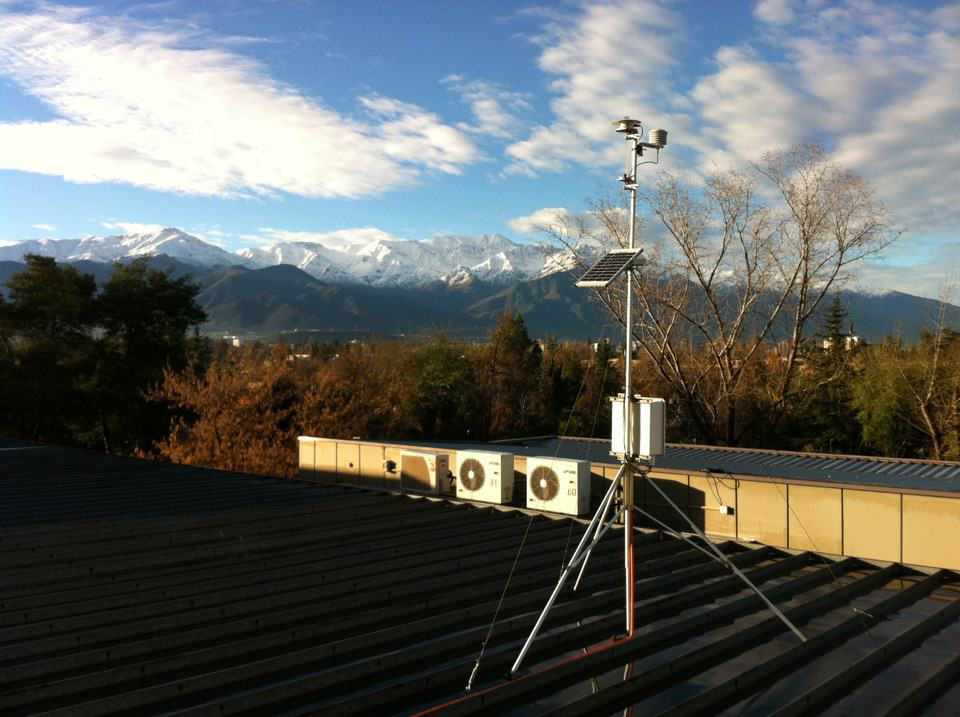
\includegraphics[scale=0.35]{images/estacionDedaloFch}
        \caption{Estación de medición de radiación solar en Fundación Chile, Vitacura - Santiago.}
	\label{fotoEstacionFch}
\end{figure}

\begin{figure}[h!]
        \centering
        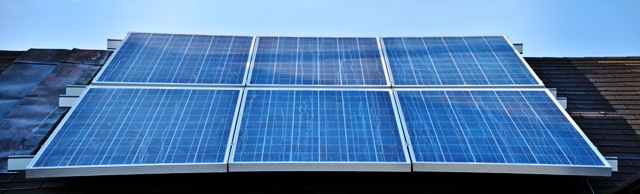
\includegraphics[scale=2.2]{images/mmena}
        \caption{Módulos solares de la planta solar de Marcelo Mena, Vitacura - Santiago.}
        \label{fotoPlantaMarcelo}
\end{figure}

Actualmente, RedSolLAC no cuenta con ningún sistema informático que le permita exponer a sus usuarios las lecturas de las estaciones y plantas solares que pertenecen a la red, por lo que es necesario implementar un sistema que permita publicar dicha información.\\

Los datos de adquisición propia provienen de una estación de medición de radiación solar, temperatura y humedad ambiente, instalada en Fundación Chile, en la comuna de Vitacura, Santiago de Chile. Esta estación (Ver. Fig.\ref{fotoEstacionFch}).

Los datos provenientes de la planta ''MarceloMena'' (Ver. Fig. \ref{fotoPlantaMarcelo}), corresponden a una pequeña planta de producción residencial con el fin de abastecer de energía a un vivienda en la comuna de Vitacura en Santiago de Chile. Estos datos son de especial interés, ya que permitirán realizar una comparación entre los resultados de la simulación entregados por la ''calculadora'' desarrollada y datos de producción empírica.

Los principales actores y usuarios de este sistema son todos los miembros de la RedSolLAC, interesados en recibir y compartir información relacionada con la energía solar fotovoltaica. En todo caso, la plataforma es abierta, por lo que cualquier otro usuario puede acceder a esta información.\\

El BID a través del proyecto RedSolLac que desarrolla la Fundación Chile espera conectar a los actores claves en el desarrollo de la energía solar fotovoltaica de Latinoamérica y el Caribe. En la actualidad, existen pocos actores en la región, por lo que el conocimiento técnico en esta materia se reduce a experiencias de universidades y algunas iniciativas privadas aisladas. RedSolLAC busca convertirse en un sitio de referencia para el estudio y desarrollo de nuevas iniciativas solares.\\

El desarrollo de esta memoria, permite a la comunidad de la RedSolLac contar con una gran base de datos para todos sus usuarios, así como diversas aplicaciones en su plataforma, para la difusión y el patrocinio de la energía solar en la región. Una red como esta, potencia el desarrollo de todas las Energías Renovables No Convencionales (\gloss{ERNC}), especialmente la fotovoltaica, esto se traduce en un beneficio medioambiental directo para toda la comunidad perteneciente a la ''red'' y a la población en general.

\section{Objetivo principal de la solución}
Desarrollar e implementar un sistema informático para la RedSolLAC, que permita interconectar equipos y estaciones de medición solar para la recolección y explotación de datos e información técnica.

\section{Objetivos específicos de la solución}
\begin{itemize}
\item Interconectar los diferentes sistemas que componen las estaciones de medición, para que exista una comunicación efectiva entre dichos sistemas y una base de datos común en Internet.
\item Desarrollo de un sistema Web capaz de procesar y publicar la información recopilada de una planta de energía solar.
\item Desarrollo de una calculadora online para sistemas fotovoltaicos, que permita dimensionar y estimar los costos de producción de energía eléctrica.
\item Realizar pruebas de la plataforma en conjunto con todos sus componentes, comparar los datos obtenidos con datos recopilados de otras fuentes. Estas pruebas permitirán validar el funcionamiento del software así como la acertividad del método de calculo y estimación eléctrica implementado en la solución.
\end{itemize}

\section{Requerimientos del sistema}
Para el desarrollo del sistema planteado, el BID, RedSolLAC y Fundación Chile han establecido una serie de requerimientos de diferente naturaleza los cuales se detallan en el cuadro \ref{tablaFuncional} y \ref{tablaNoFuncional}, además la figura \ref{fig:demanda} se presenta como una idea de presentación de datos originados por las estaciones y que deben ser presentadas de forma interactiva en el sitio Web de RedSolLAC.

\begin{figure}[h!]
        \centering
        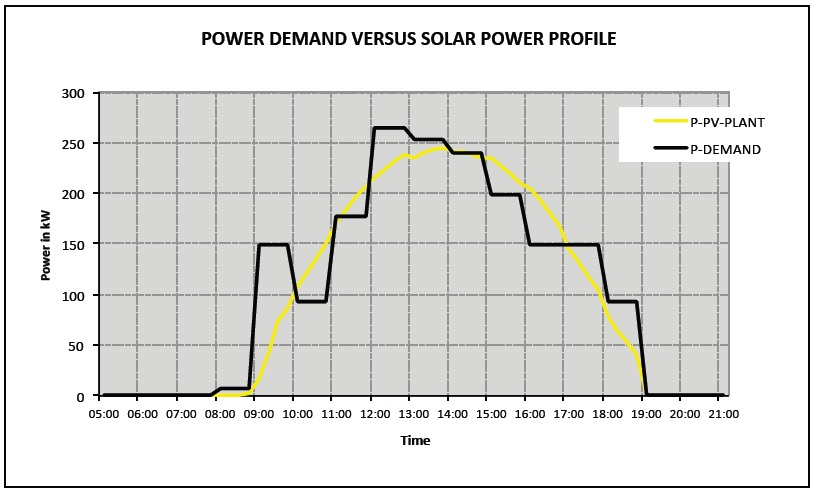
\includegraphics[scale=0.35]{images/demandaGeneracionSubSole}
        \caption{Gráfico de ejemplo de la curva de generación de energía solar.}
	\label{fig:demanda}
\end{figure}
\newpage

\subsection{Requerimientos funcionales}
\begin{table}[h!]
\caption{Tabla de requerimientos funcionales}
\label{tablaFuncional}
\begin{tabular}{| c | p{11cm} |}
	\hline
	\textbf{Requerimiento}	&	\textbf{Detalle}	\\
	\hline
	RF-1	&	Registro de datos en linea, las estaciones deben ser programadas para registrar los datos capturados en una base de datos externa en internet, el registro de datos debe ser cada 1 minuto.	\\
	\hline
	RF-2	&	La aplicación debe ser capas de visualizar datos actuales históricos e instantáneos, se debe proporcionar un modulo de visualización de datos que permita al usuario apreciar de manera total o parcial los datos registrados por las estaciones, permitiendo seleccionar periodos de tiempo y diferentes tipos de datos proporcionados por los sensores que conforman la estación.\\
	\hline
	RF-3	&	Descarga de datos, los datos registrados por las estaciones deben estar disponibles para su descarga en un formato practico para la utilización de estos por usuarios expertos, pudiendo estos usuarios descargar datos de acuerdo a un periodo de tiempo especificado.	\\
	\hline
	RF-4	&	Permitir el ingreso de información, la aplicación debe permitir el ingreso de parámetros geográficos, información técnica de planta y datos económicos para realizar los cálculos del dimensionamiento de una planta de energía solar 	\\
	\hline
	RF-5	&	Implementar un modelo de calculo de energía horario basado en el documento ''Modelo de radiación solar para conversión de datos sintéticos de radiación solar en valores horarios'', extracto de la memoria de ''master'' ''Dimensionamiento para sistemas solar térmicos en la república de Chile\cite{memoriaEdu}'' (Ver anexo \ref{memoriaEdu2})\\
	\hline
	RF-6	&	Calcular y exponer resultados de producción energética, los resultados deben ser verificables y comparables con otros sistemas, los cálculos deben presentar errores no superiores al 5\%	\\
	\hline
\end{tabular}
\end{table}

\subsection{requerimientos no funcionales}
\begin{table}[h!]
\caption{Tabla de requerimientos no funcionales}
\label{tablaNoFuncional}
\begin{tabular}{| c | p{11cm} |}
	\hline
	\textbf{Requerimiento}	&	\textbf{Detalle}	\\
	\hline
	RNF-1	&	La aplicación debe ser independiente del Sistema operativo y del navegador utilizado por el usuarios final	\\
	\hline
	RNF-2	&	Es necesario que la aplicación se integre con la imagen corporativa de la RedSolLac	\\
	\hline
	RNF-3	&	El sistema debe entregar estabilidad y muy alta confiabilidad en el registro y almacenamiento de datos	\\
	\hline
	RNF-4	&	La aplicación debe ser portable y fácilmente adaptable para funcionar con múltiples fuentes de datos 	\\
	\hline
	RNF-5	&	La aplicación debe proporcionar un mínimo estándar de seguridad que permita asegurar la confiabilidad de los datos	\\
	\hline
	RNF-6	&	La aplicación debe entregar un resultado al usuario final en tiempo aceptable no mayor a 5 seg	\\
	\hline
\end{tabular}
\end{table}


